\documentclass[border=10pt]{standalone}
\usepackage{times}
\usepackage{tikz}
\usetikzlibrary{positioning, arrows.meta, fit, backgrounds}
\begin{document}
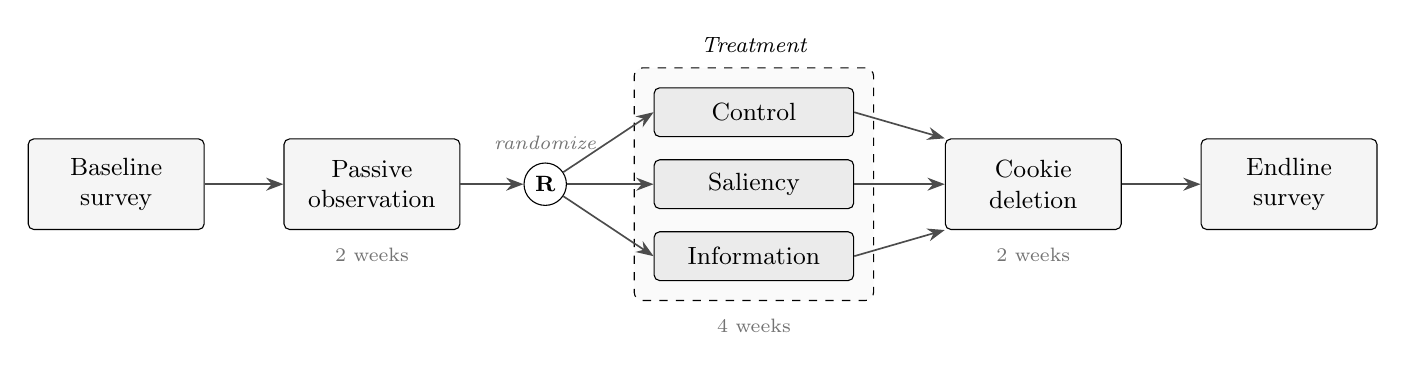
\begin{tikzpicture}[
  font=\small,
  >={Stealth[length=2.2mm]},
  phase/.style={draw, rounded corners=2pt, align=center, minimum height=1.15cm,
                text width=2.0cm, fill=black!4},
  arm/.style={draw, rounded corners=2pt, align=center, minimum height=0.62cm,
              text width=2.3cm, fill=black!8},
  arr/.style={->, semithick, draw=black!70},
  dur/.style={font=\scriptsize, text=black!55},
]
% ---- main timeline ----
\node[phase] (base) {Baseline\\survey};
\node[phase, right=1.0cm of base] (obs) {Passive\\observation};
\node[circle, draw, fill=white, right=0.8cm of obs, inner sep=2.2pt,
      font=\footnotesize\bfseries] (rand) {R};
% ---- treatment arms ----
\node[arm, right=1.1cm of rand] (sal) {Saliency};
\node[arm, above=0.28cm of sal] (ctrl) {Control};
\node[arm, below=0.28cm of sal] (info) {Information};
\node[phase, right=1.15cm of sal] (cookie) {Cookie\\deletion};
\node[phase, right=1.0cm of cookie] (end) {Endline\\survey};
% ---- treatment grouping box ----
\begin{scope}[on background layer]
  \node[draw, dashed, rounded corners=3pt, fit=(ctrl)(info),
        inner sep=7pt, fill=black!2] (trt) {};
\end{scope}
\node[above=2pt of trt.north, font=\footnotesize\itshape] {Treatment};
% ---- arrows ----
\draw[arr] (base) -- (obs);
\draw[arr] (obs) -- (rand);
\draw[arr] (rand) -- (ctrl.west);
\draw[arr] (rand) -- (sal.west);
\draw[arr] (rand) -- (info.west);
\draw[arr] (ctrl.east) -- (cookie.north west);
\draw[arr] (sal.east)  -- (cookie.west);
\draw[arr] (info.east) -- (cookie.south west);
\draw[arr] (cookie) -- (end);
% ---- durations ----
\node[dur, below=3pt of obs] {2 weeks};
\node[dur, below=3pt of trt.south] {4 weeks};
\node[dur, below=3pt of cookie] {2 weeks};
% ---- randomize note ----
\node[font=\scriptsize\itshape, text=black!55, above=1pt of rand] {randomize};
\end{tikzpicture}
\end{document}
